\documentclass{beamer}
\usepackage[utf8]{inputenc}
\usepackage[T1]{fontenc}
\usepackage{graphicx}
\usepackage{xcolor}
\usepackage{listings}
\usepackage{tikz}
\usepackage{amsmath}
\usepackage{hyperref}
\usepackage{bookmark}

% Theme - Import oppstar theme from beamer-template directory
% Add beamer-template directory to LaTeX search path
\makeatletter
\def\input@path{{./beamer-template/}}
\makeatother

% Now load the theme components
\usepackage{./beamer-template/beamercolorthemeoppstar}
\usepackage{./beamer-template/beamerfontthemeoppstar}
\usepackage{./beamer-template/beamerinnerthemeoppstar}
\usepackage{./beamer-template/beamerouterthemeoppstar}
\usepackage{./beamer-template/beamerthemeoppstar}

% Colors
\definecolor{codeblue}{RGB}{0,102,204}
\definecolor{codegray}{RGB}{128,128,128}
\definecolor{codegreen}{RGB}{0,128,0}
\definecolor{backcolour}{RGB}{245,245,245}

% Code listing style
\lstdefinestyle{cstyle}{
    backgroundcolor=\color{backcolour},
    commentstyle=\color{codegreen},
    keywordstyle=\color{codeblue},
    numberstyle=\tiny\color{codegray},
    stringstyle=\color{red},
    basicstyle=\ttfamily\footnotesize,
    breakatwhitespace=false,
    breaklines=true,
    keepspaces=true,
    numbers=left,
    numbersep=5pt,
    showspaces=false,
    showstringspaces=false,
    showtabs=false,
    tabsize=2,
    frame=single
}

\lstset{style=cstyle}

% Title page info
\title{Day 6: Capstone Project and Course Synthesis}
\subtitle{C Programming for Post-Silicon Validation Engineers}
\author{Yahwista Salomo}
\date{6-Day Intensive Bootcamp}
\institute{Post-Silicon Validation Training Program}

\begin{document}

\frame{\titlepage}

\begin{frame}
\frametitle{Welcome to Day 6!}
\begin{center}
\Large The Grand Finale: Your Validation Masterpiece
\end{center}

\begin{itemize}
    \item \footnotesize \textbf{Journey So Far:} From zero to embedded validation expert
    \item \footnotesize \textbf{Today's Mission:} Integrate everything into a capstone project
    \item \footnotesize \textbf{Validation Focus:} Simple embedded system with hardware interaction
    \item \footnotesize \textbf{Team Collaboration:} Work together on beginner-friendly projects
    \item \footnotesize \textbf{Outcome:} Professional portfolio and presentation!
\end{itemize}

\vspace{0.5cm}
\begin{center}
\textit{``Success is the sum of small efforts repeated day in and day out''} - Robert Collier
\end{center}
\end{frame}

\begin{frame}
\frametitle{Your Amazing Journey}
\begin{center}
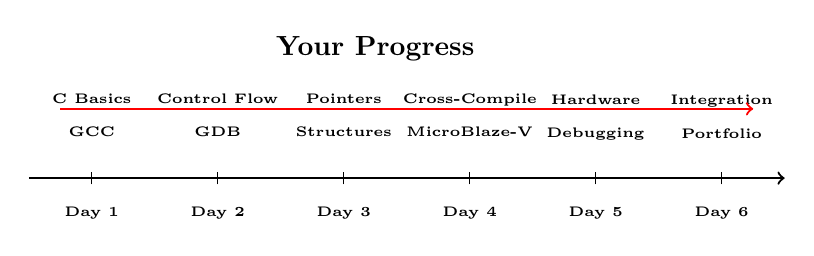
\begin{tikzpicture}[scale=0.8]
% Timeline
\draw[thick, ->] (0,0) -- (12,0);

% Day markers
\foreach \x/\day in {1/\tiny \textbf{Day 1}, 3/\tiny \textbf{Day 2}, 5/\tiny \textbf{Day 3}, 7/\tiny \textbf{Day 4}, 9/\tiny \textbf{Day 5}, 11/\tiny \textbf{Day 6}} {
    \draw (\x,-0.1) -- (\x,0.1);
    \node[below] at (\x,-0.3) {\day};
}

% Skills acquired
\node[above, align=center] at (1,0.5) {\tiny \textbf{C Basics}\\\tiny \textbf{GCC}};
\node[above, align=center] at (3,0.5) {\tiny \textbf{Control Flow}\\\tiny \textbf{GDB}};
\node[above, align=center] at (5,0.5) {\tiny \textbf{Pointers}\\\tiny \textbf{Structures}};
\node[above, align=center] at (7,0.5) {\tiny \textbf{Cross-Compile}\\\tiny \textbf{MicroBlaze-V}};
\node[above, align=center] at (9,0.45) {\tiny \textbf{Hardware}\\\tiny \textbf{Debugging}};
\node[above, align=center] at (11,0.48) {\tiny \textbf{Integration}\\\tiny \textbf{Portfolio}};

% Progress arrow
\draw[thick, red, ->] (0.5,1.1) -- (11.5,1.1);
\node[above] at (5.5,1.7) {\textbf{Your Progress}};
\end{tikzpicture}
\end{center}

\vspace{0.3cm}
\textbf{What you've mastered:}
\begin{itemize}
    \item C programming fundamentals and advanced concepts
    \item Professional development tools and workflows
    \item Embedded systems programming for AMD Microblaze-V
    \item Hardware validation techniques and best practices
    \item AI-assisted development and critical evaluation
\end{itemize}
\end{frame}

\begin{frame}
\frametitle{Today's Learning Objectives}
By the end of Day 6, you will:

\begin{enumerate}
    \item Integrate all course concepts into a comprehensive project
    \item Demonstrate professional project management skills
    \item Create and deliver technical presentations
    \item Build a portfolio-ready GitHub repository
    \item Plan your continued learning journey
    \item Network with peers and establish professional connections
\end{enumerate}

\vspace{0.5cm}
\begin{alertblock}{Capstone Day}
Today you prove you're ready for post-silicon validation roles!
\end{alertblock}
\end{frame}

\begin{frame}
\frametitle{Capstone Project Overview}
\footnotesize \textbf{Project Goal:} Build a simple embedded application using pre-configured AMD Microblaze-V FPGA boards that demonstrates core C programming and hardware interaction concepts.

\vspace{0.3cm}
\textbf{Team Structure:}
\begin{itemize}
    \item \footnotesize Teams of 2-3 participants
    \item \footnotesize Each team gets a pre-configured FPGA board
    \item \footnotesize Collaborative development using provided templates
    \item \footnotesize Focus on learning rather than complex system design
\end{itemize}

\vspace{0.3cm}
\textbf{Time Allocation:}
\begin{itemize}
    \item \footnotesize \textbf{Setup \& Exploration:} 1 hour
    \item \footnotesize \textbf{Implementation:} 3 hours
    \item \footnotesize \textbf{Testing \& Documentation:} 1.5 hours
    \item \footnotesize \textbf{Presentations:} 1.5 hours
\end{itemize}
\end{frame}

\begin{frame}
\frametitle{Project Requirements}
\textbf{Core Requirements (Must Have):}
\begin{enumerate}
    \item \footnotesize Basic peripheral interaction (UART, GPIO, Timer)
    \item \footnotesize Simple modular code structure
    \item \footnotesize Cross-compilation for Microblaze-V using provided Makefile
    \item \footnotesize Basic hardware testing on FPGA board
    \item \footnotesize Simple error handling
    \item \footnotesize Basic documentation and comments
\end{enumerate}

\vspace{0.3cm}
\textbf{Optional Features (Choose 1-2):}
\begin{itemize}
    \item \footnotesize LED blinking patterns or simple displays
    \item \footnotesize Basic sensor reading (if available on board)
    \item \footnotesize Simple user interaction via UART console
    \item \footnotesize Basic timing measurements
    \item \footnotesize Simple data logging or reporting
    \item \footnotesize Creative use of available peripherals
\end{itemize}
\end{frame}

\begin{frame}
\frametitle{Project Ideas and Inspiration}
\small \textbf{Suggested Project Themes:}

\begin{enumerate}
    \item \footnotesize \textbf{LED Pattern Controller:} Create different blinking patterns and sequences
    \item \footnotesize \textbf{UART Echo System:} Simple console that echoes user input with processing
    \item \footnotesize \textbf{Timer-Based Stopwatch:} Measure and display elapsed time
    \item \footnotesize \textbf{GPIO Input Monitor:} Read switches/buttons and display status
    \item \footnotesize \textbf{Simple Data Logger:} Log sensor readings or user inputs
    \item \footnotesize \textbf{Basic Calculator:} Simple arithmetic via UART interface
\end{enumerate}

\vspace{0.3cm}
\small \textbf{Keep It Simple:}
\begin{itemize}
    \item \footnotesize Focus on one main feature
    \item \footnotesize Use provided code templates
    \item \footnotesize Build incrementally
    \item \footnotesize Test frequently on hardware
\end{itemize}
\end{frame}

\begin{frame}[fragile]
\frametitle{Project Architecture Template}
\begin{lstlisting}[basicstyle=\tiny\ttfamily]
Simple project structure:
microblaze_project/
|-- src/
|   |-- main.c                 // Main application
|   |-- peripherals.c          // UART, GPIO, Timer drivers
|   +-- start.s               // Assembly startup file
|-- include/
|   +-- peripherals.h         // Hardware interface definitions
|-- linker/
|   +-- microblaze_v.ld       // Linker script (provided)
|-- Makefile                   // Build configuration (provided)
+-- README.md                  // Project documentation
\end{lstlisting}
\end{frame}

\begin{frame}[fragile]
\frametitle{Sample Capstone Code Structure}
\begin{lstlisting}[language=C, basicstyle=\tiny]
// peripherals.h - Simple hardware interface
#ifndef PERIPHERALS_H
#define PERIPHERALS_H

#include <stdint.h>

// Microblaze-V peripheral addresses
#define UARTLITE_BASE    0x40600000
#define TIMER_BASE       0x41C00000
#define GPIO_BASE        0x40000000

// UARTlite functions
void uart_putc(char c);
void uart_puts(const char *str);
char uart_getc(void);

// Timer functions
void timer_init(uint32_t reload_value);
uint32_t timer_read(void);
void delay_ms(uint32_t ms);

// GPIO functions
void gpio_set_output(uint32_t pin, uint32_t value);
uint32_t gpio_read_input(uint32_t pin);

#endif // PERIPHERALS_H
\end{lstlisting}
\end{frame}

\begin{frame}
\frametitle{Team Formation and Roles}
\small \textbf{Team Formation Strategy:}
\begin{itemize}
    \item \footnotesize Mix of different skill levels and backgrounds
    \item \footnotesize Complementary strengths (hardware focus, software focus, etc.)
    \item \footnotesize Good communication and collaboration potential
    \item \footnotesize Shared interest in project theme
\end{itemize}

\vspace{0.3cm}
\small \textbf{Suggested Roles:}
\begin{itemize}
    \item \footnotesize \textbf{Project Lead:} Overall coordination and integration
    \item \footnotesize \textbf{Hardware Specialist:} Microblaze-V programming and debugging
    \item \footnotesize \textbf{Software Architect:} Code structure and optimization
    \item \footnotesize \textbf{Quality Engineer:} Testing and validation
    \item \footnotesize \textbf{Documentation Lead:} README, comments, and presentation
\end{itemize}

\vspace{0.3cm}
\textbf{Note:} In 2-3 person teams, members wear multiple hats!
\end{frame}

\begin{frame}
\frametitle{Project Planning Session}
\small \textbf{Planning Checklist (30 minutes):}

\begin{enumerate}
    \item \footnotesize \textbf{Project Selection:} Choose theme and scope
    \item \footnotesize \textbf{Requirements Definition:} Core and advanced features
    \item \footnotesize \textbf{Architecture Design:} Module breakdown and interfaces
    \item \footnotesize \textbf{Task Assignment:} Who does what and when
    \item \footnotesize \textbf{GitHub Setup:} Repository creation and branch strategy
    \item \footnotesize \textbf{Milestone Planning:} Hourly checkpoints and deliverables
\end{enumerate}

\vspace{0.3cm}
\small \textbf{Planning Tools:}
\begin{itemize}
    \item \footnotesize GitHub Projects for task tracking
    \item \footnotesize Shared Google Doc for design notes
    \item \footnotesize Whiteboard for architecture diagrams
    \item \footnotesize Timer for milestone management
\end{itemize}
\end{frame}

\begin{frame}
\frametitle{Development Best Practices}
\small \textbf{Collaborative Development:}
\begin{itemize}
    \item \footnotesize \textbf{Frequent commits:} Small, focused changes
    \item \footnotesize \textbf{Descriptive messages:} Clear commit descriptions
    \item \footnotesize \textbf{Branch strategy:} Feature branches with pull requests
    \item \footnotesize \textbf{Code reviews:} Peer review before merging
    \item \footnotesize \textbf{Continuous integration:} Automated testing
\end{itemize}

\vspace{0.3cm}
\small \textbf{Quality Assurance:}
\begin{itemize}
    \item \footnotesize \textbf{Unit testing:} Test individual functions
    \item \footnotesize \textbf{Integration testing:} Test module interactions
    \item \footnotesize \textbf{Hardware testing:} Validate on actual Microblaze-V
    \item \footnotesize \textbf{Performance testing:} Measure execution times
    \item \footnotesize \textbf{Documentation:} Keep README updated
\end{itemize}
\end{frame}

\begin{frame}
\frametitle{AI Integration Guidelines}
\small \textbf{Responsible AI Usage:}
\begin{itemize}
    \item \footnotesize \textbf{Code Generation:} Use AI for boilerplate and complex algorithms
    \item \footnotesize \textbf{Optimization:} Ask AI for performance improvement suggestions
    \item \footnotesize \textbf{Debugging:} Get AI help with error analysis
    \item \footnotesize \textbf{Documentation:} AI-assisted comment and README generation
    \item \footnotesize \textbf{Testing:} AI-generated test cases and edge conditions
\end{itemize}

\vspace{0.3cm}
\small \textbf{Documentation Requirements:}
\begin{itemize}
    \item \footnotesize Note all AI assistance in commit messages
    \item \footnotesize Include AI evaluation section in README
    \item \footnotesize Explain why AI suggestions were accepted/rejected
    \item \footnotesize Demonstrate understanding of AI-generated code
    \item \footnotesize Show improvements made to AI suggestions
\end{itemize}
\end{frame}

\begin{frame}
\frametitle{Presentation Guidelines}
\small \textbf{Presentation Structure (7-10 minutes):}
\begin{enumerate}
    \item \footnotesize \textbf{Introduction (1 min):} Team and project overview
    \item \footnotesize \textbf{Problem Statement (1 min):} What validation challenge you solved
    \item \footnotesize \textbf{Solution Architecture (2 min):} High-level design and approach
    \item \footnotesize \textbf{Technical Implementation (3 min):} Key code and algorithms
    \item \footnotesize \textbf{Demonstration (2 min):} Live demo on Microblaze-V hardware
    \item \footnotesize \textbf{Results \& Lessons (1 min):} What worked, what you learned
\end{enumerate}

\vspace{0.5cm}
\small \textbf{Presentation Tips:}
\begin{itemize}
    \item \footnotesize Focus on validation engineering relevance
    \item \footnotesize Show actual code and hardware
    \item \footnotesize Highlight innovative features
    \item \footnotesize Discuss challenges and solutions
    \item \footnotesize Demonstrate professional communication
\end{itemize}
\end{frame}

\begin{frame}
\frametitle{Evaluation Criteria}
\begin{columns}[T]
\begin{column}{0.5\textwidth}
\tiny \textbf{Technical Implementation (40\%):}

\begin{itemize}\tiny
    \item \tiny Code quality and organization
    \item \tiny Proper use of course concepts
    \item \tiny Hardware integration effectiveness
    \item \tiny Error handling and robustness
\end{itemize}

\tiny \textbf{Innovation \& Problem Solving (25\%):}
\begin{itemize}\tiny
    \item \tiny Creative approach to validation challenges
    \item \tiny Advanced feature implementation
    \item \tiny Novel use of Microblaze-V capabilities
    \item \tiny AI integration effectiveness
\end{itemize}
\end{column}

\begin{column}{0.5\textwidth}
\tiny \textbf{Collaboration \& Process (20\%):}
\begin{itemize}\tiny
    \item \tiny GitHub workflow and commit quality
    \item \tiny Team collaboration effectiveness
    \item \tiny Code review participation
    \item \tiny Project management skills
\end{itemize}

\tiny \textbf{Communication \& Documentation (15\%):}
\begin{itemize}\tiny
    \item \tiny Presentation quality and clarity
    \item \tiny Documentation completeness
    \item \tiny Professional communication
    \item \tiny Technical explanation accuracy
\end{itemize}
\end{column}
\end{columns}
\end{frame}

\begin{frame}
\frametitle{Portfolio Development}
\small \textbf{Your GitHub Portfolio Should Include:}
\begin{itemize}
    \item \footnotesize \textbf{Professional README:} Clear project description and setup
    \item \footnotesize \textbf{Code Quality:} Well-commented, organized source code
    \item \footnotesize \textbf{Documentation:} API reference and user guides
    \item \footnotesize \textbf{Demonstration:} Videos or GIFs of hardware in action
    \item \footnotesize \textbf{Technical Writing:} Design decisions and trade-offs
    \item \footnotesize \textbf{Professional Profile:} Updated GitHub profile and bio
\end{itemize}

\vspace{0.3cm}
\textbf{Career Integration:}
\begin{itemize}
    \item \footnotesize Link to LinkedIn profile
    \item \footnotesize Highlight validation engineering skills
    \item \footnotesize Showcase embedded systems experience
    \item \footnotesize Demonstrate collaborative development
    \item \footnotesize Show continuous learning mindset
\end{itemize}
\end{frame}

\begin{frame}
\frametitle{Milestone Checkpoints}
\small \textbf{Hourly Progress Checks:}

\begin{itemize}
    \item \footnotesize \textbf{Hour 1:} Planning complete, GitHub setup, initial code structure
    \item \footnotesize \textbf{Hour 2:} Basic peripheral drivers working (UART output)
    \item \footnotesize \textbf{Hour 3:} Core functionality implemented and tested
    \item \footnotesize \textbf{Hour 4:} Optional features added, basic optimization
    \item \footnotesize \textbf{Hour 5:} Testing complete, documentation finalized
    \item \footnotesize \textbf{Hour 6:} Presentation prepared, final demo ready
\end{itemize}

\vspace{0.3cm}
\small \textbf{Checkpoint Activities:}
\begin{itemize}
    \item \footnotesize Quick team standup (5 minutes)
    \item \footnotesize Progress demonstration to instructors
    \item \footnotesize Peer team check-ins and help
    \item \footnotesize Adjustment of goals if needed
    \item \footnotesize Celebration of achievements!
\end{itemize}
\end{frame}

\begin{frame}
\frametitle{Troubleshooting and Support}
\textbf{Common Challenges and Solutions:}
\begin{itemize}
    \item \footnotesize \textbf{Hardware Issues:} Backup Microblaze-V boards available
    \item \footnotesize \textbf{Compilation Problems:} TAs for build system help
    \item \footnotesize \textbf{Git Conflicts:} Pair programming and merge assistance
    \item \footnotesize \textbf{Time Management:} Scope adjustment guidance
    \item \footnotesize \textbf{Team Dynamics:} Instructor mediation if needed
\end{itemize}

\vspace{0.3cm}
\textbf{Support Resources:}
\begin{itemize}
    \item \footnotesize Instructor and TA availability throughout the day
    \item \footnotesize Peer teams for cross-pollination of ideas
    \item \footnotesize Course materials and examples for reference
    \item \footnotesize AI tools for coding assistance
    \item \footnotesize Emergency backup plans for critical issues
\end{itemize}
\end{frame}

\begin{frame}
\frametitle{Beyond the Course: Your Next Steps}
\textbf{Immediate Next Steps (Week 1-2):}
\begin{itemize}
    \item Complete post-course project enhancements
    \item Update LinkedIn with new skills and projects
    \item Connect with classmates and instructors
    \item Apply learnings to current work projects
    \item Start exploring advanced embedded topics
\end{itemize}

\vspace{0.5cm}
\textbf{Medium-term Goals (Month 1-3):}
\begin{itemize}
    \item Complete extended homework assignments
    \item Contribute to open-source embedded projects
    \item Attend embedded systems meetups and conferences
    \item Pursue advanced certifications
    \item Build additional portfolio projects
\end{itemize}

\vspace{0.5cm}
\textbf{Long-term Career Development:}
\begin{itemize}
    \item Transition to post-silicon validation roles
    \item Become a mentor for future course participants
    \item Develop expertise in specialized validation areas
    \item Lead validation teams and projects
\end{itemize}
\end{frame}

\begin{frame}
\frametitle{Course Reflection and Feedback}
\textbf{Reflection Questions:}
\begin{itemize}
    \item What was your biggest learning breakthrough?
    \item Which concepts do you want to explore further?
    \item How will you apply these skills in your career?
    \item What would you tell someone considering this course?
    \item What additional topics would be valuable?
\end{itemize}

\vspace{0.5cm}
\textbf{Feedback Opportunities:}
\begin{itemize}
    \item Course evaluation survey (anonymous)
    \item One-on-one feedback sessions with instructors
    \item Peer feedback on collaboration and learning
    \item Suggestions for course improvements
    \item Testimonials for future marketing
\end{itemize}
\end{frame}

\begin{frame}
\frametitle{Alumni Network and Community}
\textbf{Staying Connected:}
\begin{itemize}
    \item Shared GitHub organization for projects
    \item Mentorship program (alumni helping new students)
    \item Job referral network and career support
\end{itemize}

\vspace{0.5cm}
\textbf{Giving Back:}
\begin{itemize}
    \item Volunteer as TA for future courses
    \item Share your success stories and projects
    \item Provide feedback on course improvements
    \item Mentor new engineers in your organization
    \item Contribute to course materials and examples
\end{itemize}
\end{frame}

\begin{frame}
\frametitle{Final Thoughts and Congratulations}
\begin{center}
\Large You Did It!
\end{center}

\small \textbf{What you've accomplished in 6 days:}
\begin{itemize}
    \item \footnotesize Mastered C programming from zero to advanced
    \item \footnotesize Learned professional embedded development workflows
    \item \footnotesize Built real hardware validation systems
    \item \footnotesize Developed collaborative software engineering skills
    \item \footnotesize Created a professional portfolio of projects
    \item \footnotesize Joined a community of validation engineers
\end{itemize}

\vspace{0.3cm}
\begin{center}
\textbf{You are now ready for post-silicon validation roles!}
\end{center}

\vspace{0.3cm}
\begin{center}
\textit{``The journey of a thousand miles begins with a single step''} - Lao Tzu\\
\textit{You've taken many steps this week!}
\end{center}
\end{frame}

\begin{frame}
\frametitle{Let's Build Something Amazing!}
\begin{center}
\Large Time for Your Capstone Project
\end{center}

\textbf{Remember:}
\begin{itemize}
    \item Start with simple features and build up
    \item Use the provided templates and examples
    \item Test your code frequently on the hardware
    \item Don't hesitate to ask for help when stuck
    \item Focus on learning rather than complexity
    \item Have fun and celebrate your progress!
\end{itemize}

\vspace{1cm}
\begin{center}
\textbf{Go forth and validate!}
\end{center}
\end{frame}

\end{document}
